    % specifies the documnt class. We usually use article but there are others. 
\documentclass[a4paper,12pt,oneside]{book}              

% these are standard packages used for the math symbols
\usepackage{amsmath,amssymb,amsthm, enumitem, hyperref, tabto, verbatim} 
\usepackage[T1]{fontenc}
\usepackage[utf8]{inputenc}
\usepackage[english]{babel}
\usepackage{fancyhdr}
\usepackage{wrapfig}
\usepackage[fleqn]{amsmath}
\usepackage[utf8]{inputenc}
\usepackage{graphicx}
\usepackage{float}
\usepackage[absolute,overlay]{textpos}
\graphicspath{ {./Photos/} }
\usepackage{fancyhdr}
\usepackage[top=1in,bottom=1in,right=1in,left=1in]{geometry}
\usepackage{circuitikz}
\usepackage{tikz}
\usepackage{pgfplots}
\usetikzlibrary{decorations.markings,arrows}
\usetikzlibrary{datavisualization}
\usetikzlibrary{datavisualization.formats.functions}
\pgfplotsset{compat=newest}
\usepackage{amsmath}
\usepackage{ragged2e}

% These commands below is to make sure the numbering of these are consistent with theorem
% If you are not sure what something means, delete them, build a new file and see the
% difference between the files. You can ignore this part for now.
\newtheorem{theorem}{Theorem}[section]
\newtheorem{conjecture}[theorem]{Conjecture}
\newtheorem{observation}[theorem]{Observation}
\newtheorem{definition}[theorem]{Definition}
\newtheorem{corollary}[theorem]{Corollary}
\newtheorem{lemma}[theorem]{Lemma}
\newtheorem{example}[theorem]{Example}
\newtheorem{remark}[theorem]{Remark}
\newtheorem{notation}[theorem]{Notation}


% Title of your project
\title{%
  \Huge Calculus \\
  \LARGE  Exploring \textbf{Real} Math
  }

% The author command places text right after title
\author{by \\
\Large The NUS High Math Interest Group (MIG) \\
}

\date{\Large 12th November 2022}

\begin{document}
\maketitle

\tableofcontents

%\part{An Introduction}

%\newpage
\chapter{Exploring Instantaneous Change}
\vspace{-30pt}
\large \textit{by Jiang Yuzhe}

\subsection{Derivative}
So, What is the definition of a derivative?
A derivative is the instantaneous rate of change of a function at a specific point. It can usually be represented as the slope of a graph.

\subsection{Notations}
We will be focusing on 2 types of notations that are within out school's syllabus, the Langrange notation and Leibniz notation. 
\subsubsection{Functions (Pre-calculus)}
A function takes in an \textbf{input} and returns an \textbf{output}. However, for any input, the output is \textbf{unique}. For example, if A is the input into the function, and B is an output, then B is the only output of the function. If there are more than 2 outputs for the same input, then it is not a valid function. 
\subsubsection{Lagrange vs Leibniz}
\begin{tabular}{|c|c|c|}
     \hline
     & Lagrange & Leibniz \\
     \hline
     1st order & $f'(x)$& $\frac{dy}{dx}$\\[2ex]
     \hline
     2nd order & $f''(x)$& $\frac{d^2y}{dx^2}$\\[2ex]
     \hline
     3rd order & $f'''(x)$& $\frac{d^3y}{dx^3}$\\[2ex]
     \hline
     nth orders & $f^{(n)}(x)$& $\frac{d^ny}{dx^n}$\\[2ex]
     \hline
\end{tabular}
\smallskip\\
Note that n is positive, otherwise you would be performing integration.

\subsection{Standard Differentiation Results}
\begin{align*}
    \frac{d}{dx}(c) &= 0 \quad \text{(where }c\text{ is a constant)}\\
    \frac{d}{dx}(x^n) &= nx^{n-1} \quad (n\in\mathbb{R})\\
    \frac{d}{dx}(e^x) &= e^x\\
    \frac{d}{dx}(\ln x) &= \frac{1}{x} \quad , x>0\\
    \frac{d}{dx}(\sin x) &= \cos x \quad \text{(}x\text{ is in radians)}\\
    \frac{d}{dx}(\cos x) &= -\sin x \quad \text{(}x\text{ is in radians)}
\end{align*}
\subsubsection{Chain Rule}
$$\displaystyle\frac{dy}{dx} = \frac{dy}{du} \times \frac{du}{dx}$$
\subsubsection{Product Rule}
$$\displaystyle\frac{d}{dx}(uv) = u \frac{dv}{dx}+ v\frac{du}{dx}$$
\subsubsection{Quotient Rule}
$$\displaystyle\frac{d}{dx}\left(\frac{u}{v}\right) = \frac{v\frac{du}{dx}-u\frac{dv}{dx}}{v^2}$$

\newpage
\chapter{How do Limits Work?}
\vspace{-30pt}
\large \textit{by Chong How}
\subsection{Introduction to limits}
Consider $f(x) = x+8$. When $x$ gets closer and closer to 2, $f(x) = x+8$ gets closer and closer to 10. We write \[ \lim_{x\to 2} f(x) = 10 \]
Consider $g(x) = \frac{x^2-1}{x+1}$. $g(-1)$ is undefined. But if $x\neq -1$ AND $x$ gets closer and closer to $-1$, $g(x)$ gets closer and closer to $-2$. We still write \[ \lim_{x\to -1} g(x) = -2 \]function need not be defined at $-2$ for limit to exist.\\
Let $h(x) = \frac{1}{2+\sqrt{x}}$.Then \[ \lim_{x\to 4} h(x) = \frac{1}{2+\sqrt{4}} = \frac{1}{4} \]
Qns: Do Problem set 1.
\subsection{Techniques to find Limits}
If $x$ gets sufficiently close (but not equal) to $a$, $f(x)$ gets arbitrarily to $L$, then we write  \[ \lim_{x\to a} f(x) = L \] "the limit of $f(x)$ as $x$ tends to $a$ is $L$".
\begin{theorem}
Let $c$ be a constant. If $\lim\limits_{x \to a} f(x) = L$ and $\lim\limits_{x \to a} g(x) = M$.  Then \\ 
$\lim\limits_{x \to a} cf(x) = cL$\\
$\lim\limits_{x \to a} (f(x) \pm g(x)) = L \pm M$\\
$\lim\limits_{x \to a} f(x)g(x) = LM$\\
$\lim\limits_{x \to a} \frac{f(x)}{g(x)} = \frac{L}{M}$, if M $\neq$ 0
\end{theorem}
\subsubsection*{Conjugate surds.} If there are surds, usually we use conjugate to find limit. For example, $\lim\limits_{x \to 2} \frac{\sqrt{x} - \sqrt{2}}{x-2} = \lim\limits_{x \to 2} $\:\:\:\:\:\:\:\:\:\:\:\:\:\:\:\:\:\:\:\:\: = $\lim\limits_{x \to 2} \frac{1}{\sqrt{x}+\sqrt{2}} = \frac{1}{2\sqrt{2}}$
\subsubsection{A famous limit}
\[ \lim_{\theta\to 0} \frac{\sin \theta}{\theta}  =1\] Use calculator to convince yourself!
\begin{theorem}[Squeeze Theorem]
Let f(x), g(x), h(x) be functions st.
$f(x) \leq g(x) \leq h(x) \:\: \forall x$ near a, and $\lim\limits_{x \to a} f(x) =  \lim\limits_{x \to a} h(x) = L$, then $\lim\limits_{x \to a} g(x) = L$.
\end{theorem}
For example, $\lim\limits_{x \to 0} x^2\sin(\frac{1}{x})$ (Cannot use Thm. 2.0.1). Notice that $$-x^2 \leq x^2\sin(\frac{1}{x}) \leq x^2 \:\: \forall x \in \mathbb{R}$$
and apply squeeze theorem. \qedsymbol\\
Qns: Do Problem set 2.
\subsection{Precise Definition of Limit (Optional Reading)}
$\lim\limits_{x \to a} f(x) = L$ is equivalent to \[\forall \epsilon > 0, \exists \delta > 0 \:\text{such that}\: (0<|x-a|<\delta \implies |f(x) - L|<\epsilon)\] Read more about it from bprp or Paul's online Math notes.
\subsection{Limit does not exist}
There are many cases. For example,
$\lim\limits_{x \to 0} \sqrt{x}$ and
$\lim\limits_{x \to 0} \frac{|x|}{x}$.




\newpage
\chapter{Graphically Understanding the Rules}
\vspace{-30pt}
\large \textit{by Karimi Zayan}

\section{Power rule}

\subsection{Theory}

The power Rule states that

$$\frac{d}{dx}(x^n)=nx^{n-1}$$

 \noindent The symbolic proof is as follows
$$
\begin{aligned}
\frac{d}{dx}(x^n)&=\lim_{h\to 0}\frac{(x+h)^n-x^n}{h}\\
&=\lim_{h\to 0}\frac{x^n+\binom{n}{1}x^{n-1}h+\cdots +\binom{n}{n}h^n-x^n}{h}\\
&=\lim_{h\to 0}\frac{\binom{n}{1}x^{n-1}h+\cdots +\binom{n}{n}h^n}{h}\\
&=\lim_{h\to 0}\binom{n}{1}x^{n-1}+\cdots +\binom{n}{n}h^{n-1}\\
&=nx^{n-1}
\end{aligned}
$$

 \noindent To grasp an intuitive sense of this however, we can look at a geometric diagram for the equation $f(x)=x^2$.

\begin{figure}[H]
    \begin{center}
        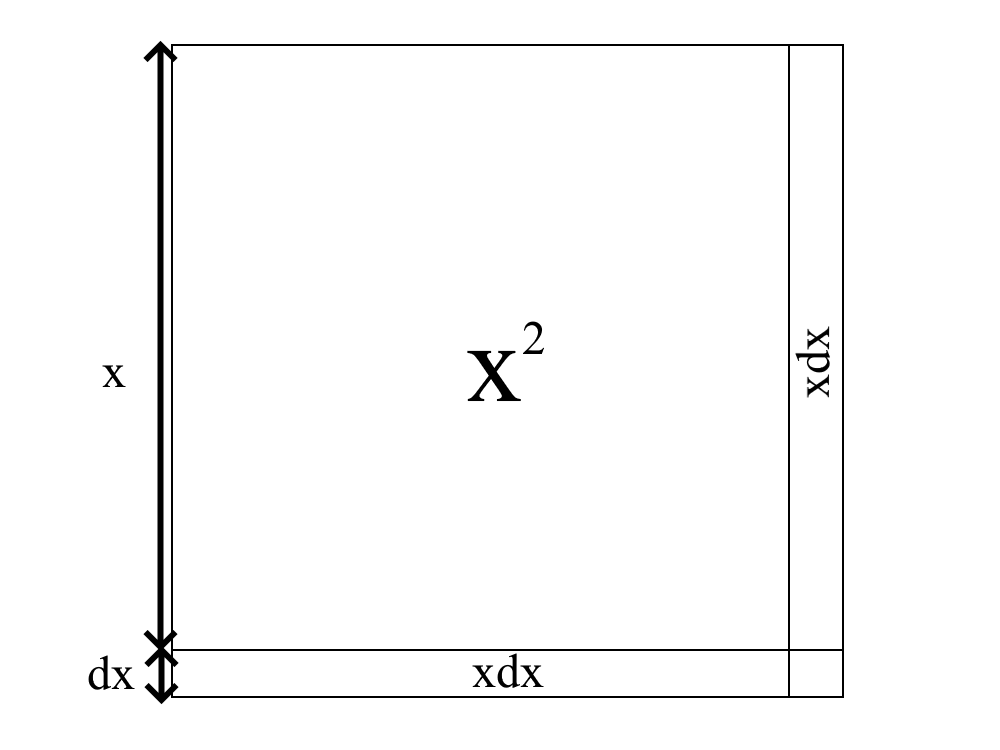
\includegraphics[scale=0.35]{img/zayan/pr1.png}
        \caption{$f=x^2$}
        \label{fig:pr1}
    \end{center}
\end{figure}

 \noindent We look at $x^2$ and if we do a small nudge to $x$ by an infinitesimally small $dx$, we get the diagram as follows. We see that we can obtain an equation for $df$ by summing up the small rectangles that make up the expression.

$$df=xdx+xdx+{dx}^2$$

 \noindent Now, we solve for $\frac{df}{dx}$,
 
$$
\begin{aligned}
df&=xdx+xdx+{dx}^2\\
\frac{df}{dx}&=2x+dx\\
\frac{df}{dx}&=2x
\end{aligned}$$

\noindent We can apply this same logic to a cube.

\begin{figure}[H]
    \begin{center}
        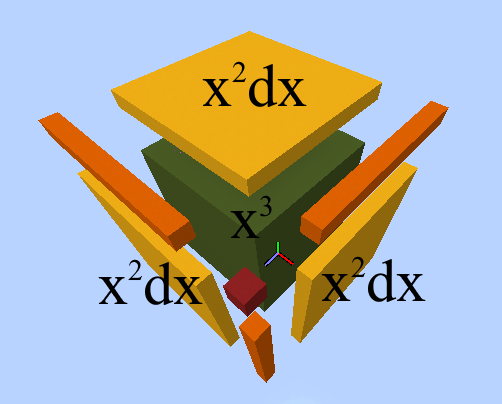
\includegraphics[scale=0.75]{img/zayan/pr2.png}
        \caption{$f=x^3$}
        \label{fig:pr2}
    \end{center}
\end{figure}

\noindent We obtain a new equation for $df$ as follows

$$df = 3x^2dx+3x{dx}^2+{dx}^3$$

\noindent We can easily see

$$\frac{df}{dx}=3x^2$$

\noindent Overall, we see that for any $x^n$, nudging $x$ by $dx$ causes there to be $n$ sections with the value $x^{n-1}dx$ and a varying amount of other sections with areas proportional to $dx^2$ which can be ignored. Hence, we can see easily now why

$$\frac{d}{dx}(x^n)=nx^{n-1}$$

\noindent The power rule defined as such applies for not just integers but also all real numbers. However, the exact proof is beyond the scope of this lesson.

\subsection{Practice Problems}

1. $x^5$

2. $5x^3$

3. $3x^1.5$

4. $\frac{3}{x}$

5. $4\sqrt{x}$

\section{Product rule}

\subsection{Theory}

The product rule states that
$$\frac{d}{dx}(f(x)g(x))=f(x)\frac{d}{dx}(g(x))+g(x)\frac{d}{dx}(f(x))$$

\noindent The symbolic proof is as follows

$$
\begin{aligned}
\frac{d}{dx}(f(x)g(x))&=\lim_{h\to 0}\frac{f(x+h)g(x+h)-f(x)g(x)}{h}\\
&=\lim_{h\to 0}\frac{{f({x+h})g({x+h})-f({x+h})g(x)+f({x+h})g(x)-f(x)g(x)}}{h}\\
&=\lim_{h\to 0}f(x+h)\frac{g(x+h)-g(x)}{h}+\lim_{h\to 0}g(x)\frac{f(x+h)-f(x)}{h}\\
&=f(x)\frac{d}{dx}(g(x))+g(x)\frac{d}{dx}(f(x))
\end{aligned}
$$

\noindent To grasp an intuitive sense of this however, we can look at a geometric diagram for the equation $y=f(x)g(x)$ similar to that of $x^2$,

\begin{figure}[H]
    \begin{center}
        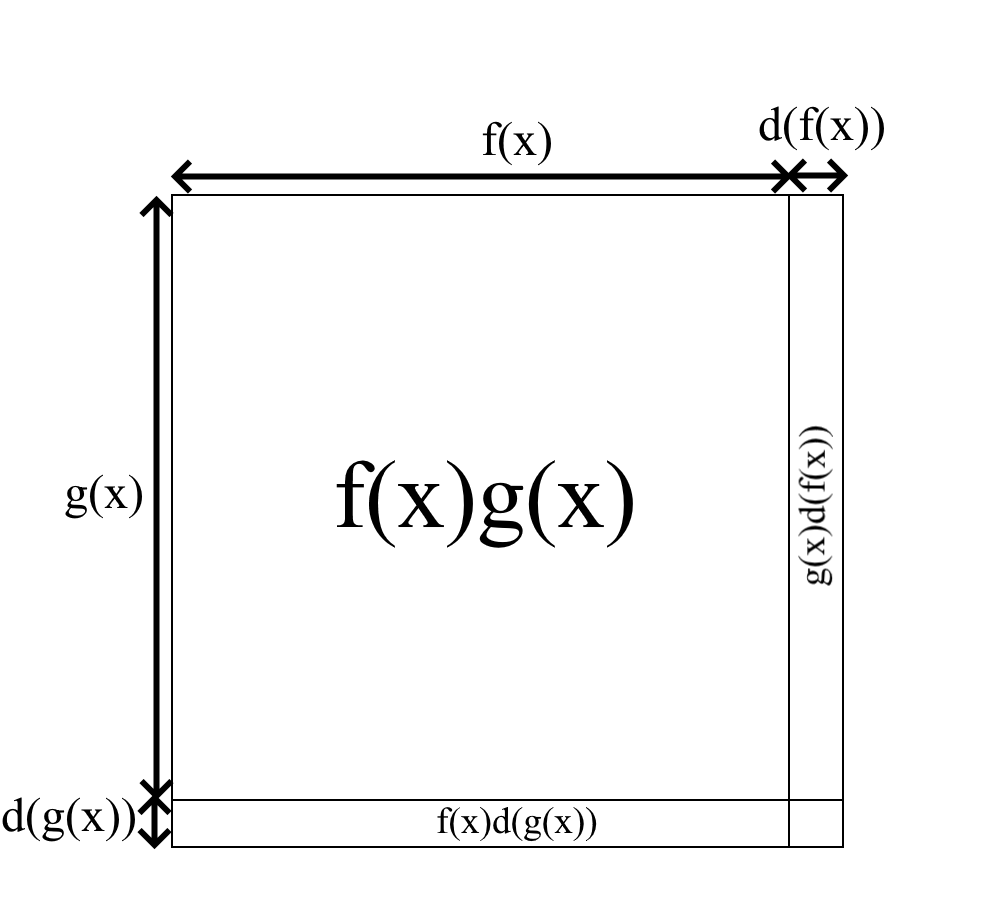
\includegraphics[scale=0.35]{img/zayan/prodrule.png}
        \caption{$y=f(x)g(x)$}
        \label{fig:prodrule}
    \end{center}
\end{figure}

\noindent We set the side lengths to be the functions, hence nudging $x$ by $dx$, the changes in the side lengths will be $d(f(x))$ and $d(g(x))$. We can obtain an expression for $dy$ by summing up all the tiny rectangles

$$dy=f(x)d(g(x))+g(x)d(f(x))+d(g(x))d(f(x))$$

\noindent we now solve for $dy$,

$$\begin{aligned}
dy&=f(x)d(g(x))+g(x)d(f(x))+d(g(x))d(f(x))\\
\frac{dy}{dx}&=f(x)\frac{d}{dx}(g(x))+g(x)\frac{d}{dx}(f(x))+\frac{d}{dx}(f(x))\frac{d}{dx}(g(x))dx\\
\frac{dy}{dx}&=f(x)\frac{d}{dx}(g(x))+g(x)\frac{d}{dx}(f(x))
\end{aligned}$$

\noindent Thus, the product rule is true.

\subsection{Practice Problems}

1. $\sin(x)x^2$

2. $x\sin(x)$

3. $x^3\ln(x)$

4. $\sin(x)\cos(x)$

5. $(\ln(x))^3$

\section{Chain rule}

\subsection{Theory}

The chain rule states that

$$\frac{d}{dx}(f(g(x)))=\frac{df(g(x))}{dg(x)}\frac{dg(x)}{dx}$$

\noindent There is no clear geometric proof for this, so I will write one. Define $u$ and $v$ as such

$$u(h)=\left\{ {\begin{array}{*{20}{l}}{\displaystyle \frac{{f( {x + h}) - f( x)}}{h} - \frac{df(x)}{dx}}&{{\mbox{  if }}h \ne 0}\\0&{{\mbox{  if }}h = 0}\end{array}} \right.$$

$$v(h)=\left\{ {\begin{array}{*{20}{l}}{\displaystyle \frac{{g( {x + h}) - g( x)}}{h} - \frac{dg(x)}{dx}}&{{\mbox{  if }}h \ne 0}\\0&{{\mbox{  if }}h = 0}\end{array}} \right.$$

\noindent We see that

$$f(x+h)=f(x)+h\left(u(h)+\frac{df(x)}{dx}\right)$$
$$g(x+h)=g(x)+h\left(v(h)+\frac{dg(x)}{dx}\right)$$

\noindent From this we can extrapolate the rule.

$$\begin{aligned}
\frac{d}{dx}(f(g(x)))&=\lim_{h\to 0}\frac{f(g(x+h))-f(g(x))}{h}\\
&=\lim_{h\to 0}\frac{f(g(x)+h\left(v(h)+\frac{dg(x)}{dx}\right))-f(g(x))}{h}\\
&=\lim_{h\to 0}\frac{f(g(x))+h\left(v(h)+\frac{dg(x)}{dx}\right)\left(u(h\left(v(h)+\frac{dg(x)}{dx}\right))+\frac{df(g(x))}{dg(x)}\right)-f(g(x))}{h}\\
&=\lim_{h\to 0}\frac{h\left(v(h)+\frac{dg(x)}{dx}\right)\left(u(h\left(v(h)+\frac{dg(x)}{dx}\right))+\frac{df(g(x))}{dg(x)}\right)}{h}\\
&=\lim_{h\to 0}\left(v(h)+\frac{dg(x)}{dx}\right)\left(u(h\left(v(h)+\frac{dg(x)}{dx}\right))+\frac{df(g(x))}{dg(x)}\right)\\
&=\frac{df(g(x))}{dg(x)}\frac{dg(x)}{dx}
\end{aligned}$$

\noindent If you don't want to read this a more simpler way to think of it is like this, if a car is moving twice as fast as a bike and a bike is moving 4 times as fast as a person. Then a car is moving 8 times faster than a person. In math form:

$$\frac{dc}{dp}=\frac{dc}{db}\frac{db}{dp}=(2)(4)=8$$

\noindent From the chain rule and product rule, we can basically calculate most derivatives since most functions are products and composites of functions with known derivatives. Hence, by recursively applying these rules, one can solve any problem.

\subsection{Practice Problems}

1. $\sin(x^2)$

2. $(\ln(x))^3$

3. $\sin^4(x^3)$

4. $\sqrt(x^5)$

5. $\sec(\tan(\sec(x)))$

\section{Quotient rule (Optional reading)}

The quotient rule states that

$$\frac{d}{dx}\left(\frac{f(x)}{g(x)}\right) = \frac{g(x)\frac{d}{dx}(f(x))-f(x)\frac{d}{dx}(g(x))}{g^2(x)}$$

\noindent We can prove this by using all the rules we have learnt so far

$$\begin{aligned}
\frac{d}{dx}\left(\frac{f(x)}{g(x)}\right)&=\frac{d}{dx}\left(f(x)\frac{1}{g(x)}\right)\\
&=f(x)\frac{d}{dx}\left(\frac{1}{g(x)}\right)+\frac{\frac{d}{dx}(f(x))}{g(x)}\\
&=-\frac{f(x)}{g^2(x)}\frac{d}{dx}(g(x))+\frac{\frac{d}{dx}(f(x))}{g(x)}\\
&=\frac{g(x)\frac{d}{dx}(f(x))-f(x)\frac{d}{dx}(g(x))}{g^2(x)}
\end{aligned}$$

%\part{Physical Applications}

\newpage
\chapter{Movement}
\vspace{-30pt}
\large \textit{by Krishna}


\newpage
\chapter{Displacement and Area Under the Curve}
\vspace{-30pt}
\large \textit{by Favian Lim and Ishan Sharma}
\newline \newline Definition of Displacement: The signed (positive, 0 or negative on a 1-dimensional line) distance away from the starting position.
\newline As stated previously, we know that v(t) = x'(t).
We could just integrate both sides to derive that the integral of v(t) dt from t=a to b is just x(b)-x(a).
\newline
\newline But there is a nicer proof using Riemann summation.

    \centering
    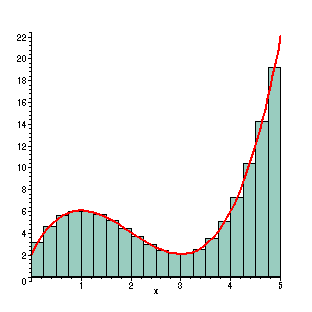
\includegraphics[width=10cm]{i_int20.png}
\justifying
\newline
\newline Let the number of rectangles used be n. In this case, n=20.
\newline As shown above, here is what Riemann summation looks like for a given curve v(t) with respect to time t. (The specific summation used is midpoint summation.) Let h be the width of each rectangle.
\newline Suppose we take the area of one rectangle. This is just the width multiplied by the height [h(f(t))], which also happens to be the displacement of the particle in the time h. If we take the sum of all the rectangles, we can get a good approximation of the area of the curve.
\newline
\newline Riemann summation is special because by letting n approach infinity and h approach 0 using limits, we also approach the exact area found under the curve, and by extension, the exact displacement of the particle.\\\\
%\newpage
%\chapter{Area under the Curve}
%\vspace{-30pt}
%\large \textit{by Ishan Sharma}
So, someone familiar with integration would know that it is often used to compute the area under a graph. However, do you know why exactly that is the case?  
\newline Take for example, the following graph: 
\begin{figure}[H]
    \begin{center}
        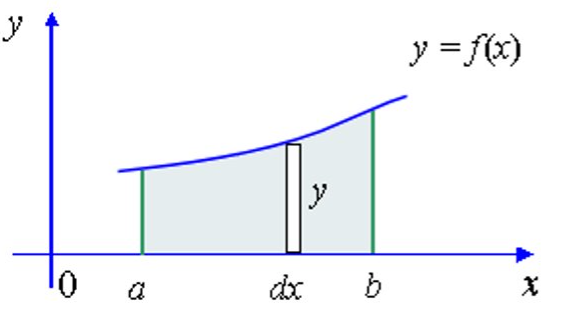
\includegraphics[scale=0.75]{img/Ishan/Image 2.png}
        \caption{Graph of y = f(x)}
        \label{fig:pr2}
    \end{center}
\end{figure}
Now, let's say you wish to calculate the area under this graph. Obviously, most graphs are not nice enough to allow you to calculate the area geometrically (for example, calculating the area under the graph of y = x just involves finding the area of a trapezium). To calculate the area of this irregular area, the area needs to be split into smaller rectangles of infinitesimal width - that is, rectangles that have a finite height but a very very small width. For such small widths, the value of y can be assumed to remain constant across the width. We call this width "dx", which means an infinitesimal change in x. \newline \newline To find the total area, all of these rectangles (with different heights) can be added together. The area of each rectangle is given by f(x) * dx. As such, we are "integrating" all the rectangles together to form a bigger area. This addition of all the triangles can be thought of the process that occurs in \(\int_{a}^{b} f(x) \,dx\). Hence, this is why integration can be used to find the area under any curve (which is integrable). 

\begin{comment}
\part{Extensions}

\newpage
\chapter{Substituting}
\vspace{-30pt}
\large \textit{by Prannaya Gupta}

Differentiation and Integration often stems from a collective understanding of how small differentials change.

This is known as the 
\end{comment}



\end{document}
